\chapter{SYSTEM DESIGN}
System design translates the requirements identified in the analysis phase into a concrete architectural framework. This chapter covers the datasets used, the preprocessing pipeline that conditions raw spectral data for learning, the three deep learning architectures at the core of the system, and the supervised, semi-supervised, and federated training paradigms evaluated against one another.

\begin{figure}[H]
    \centering
    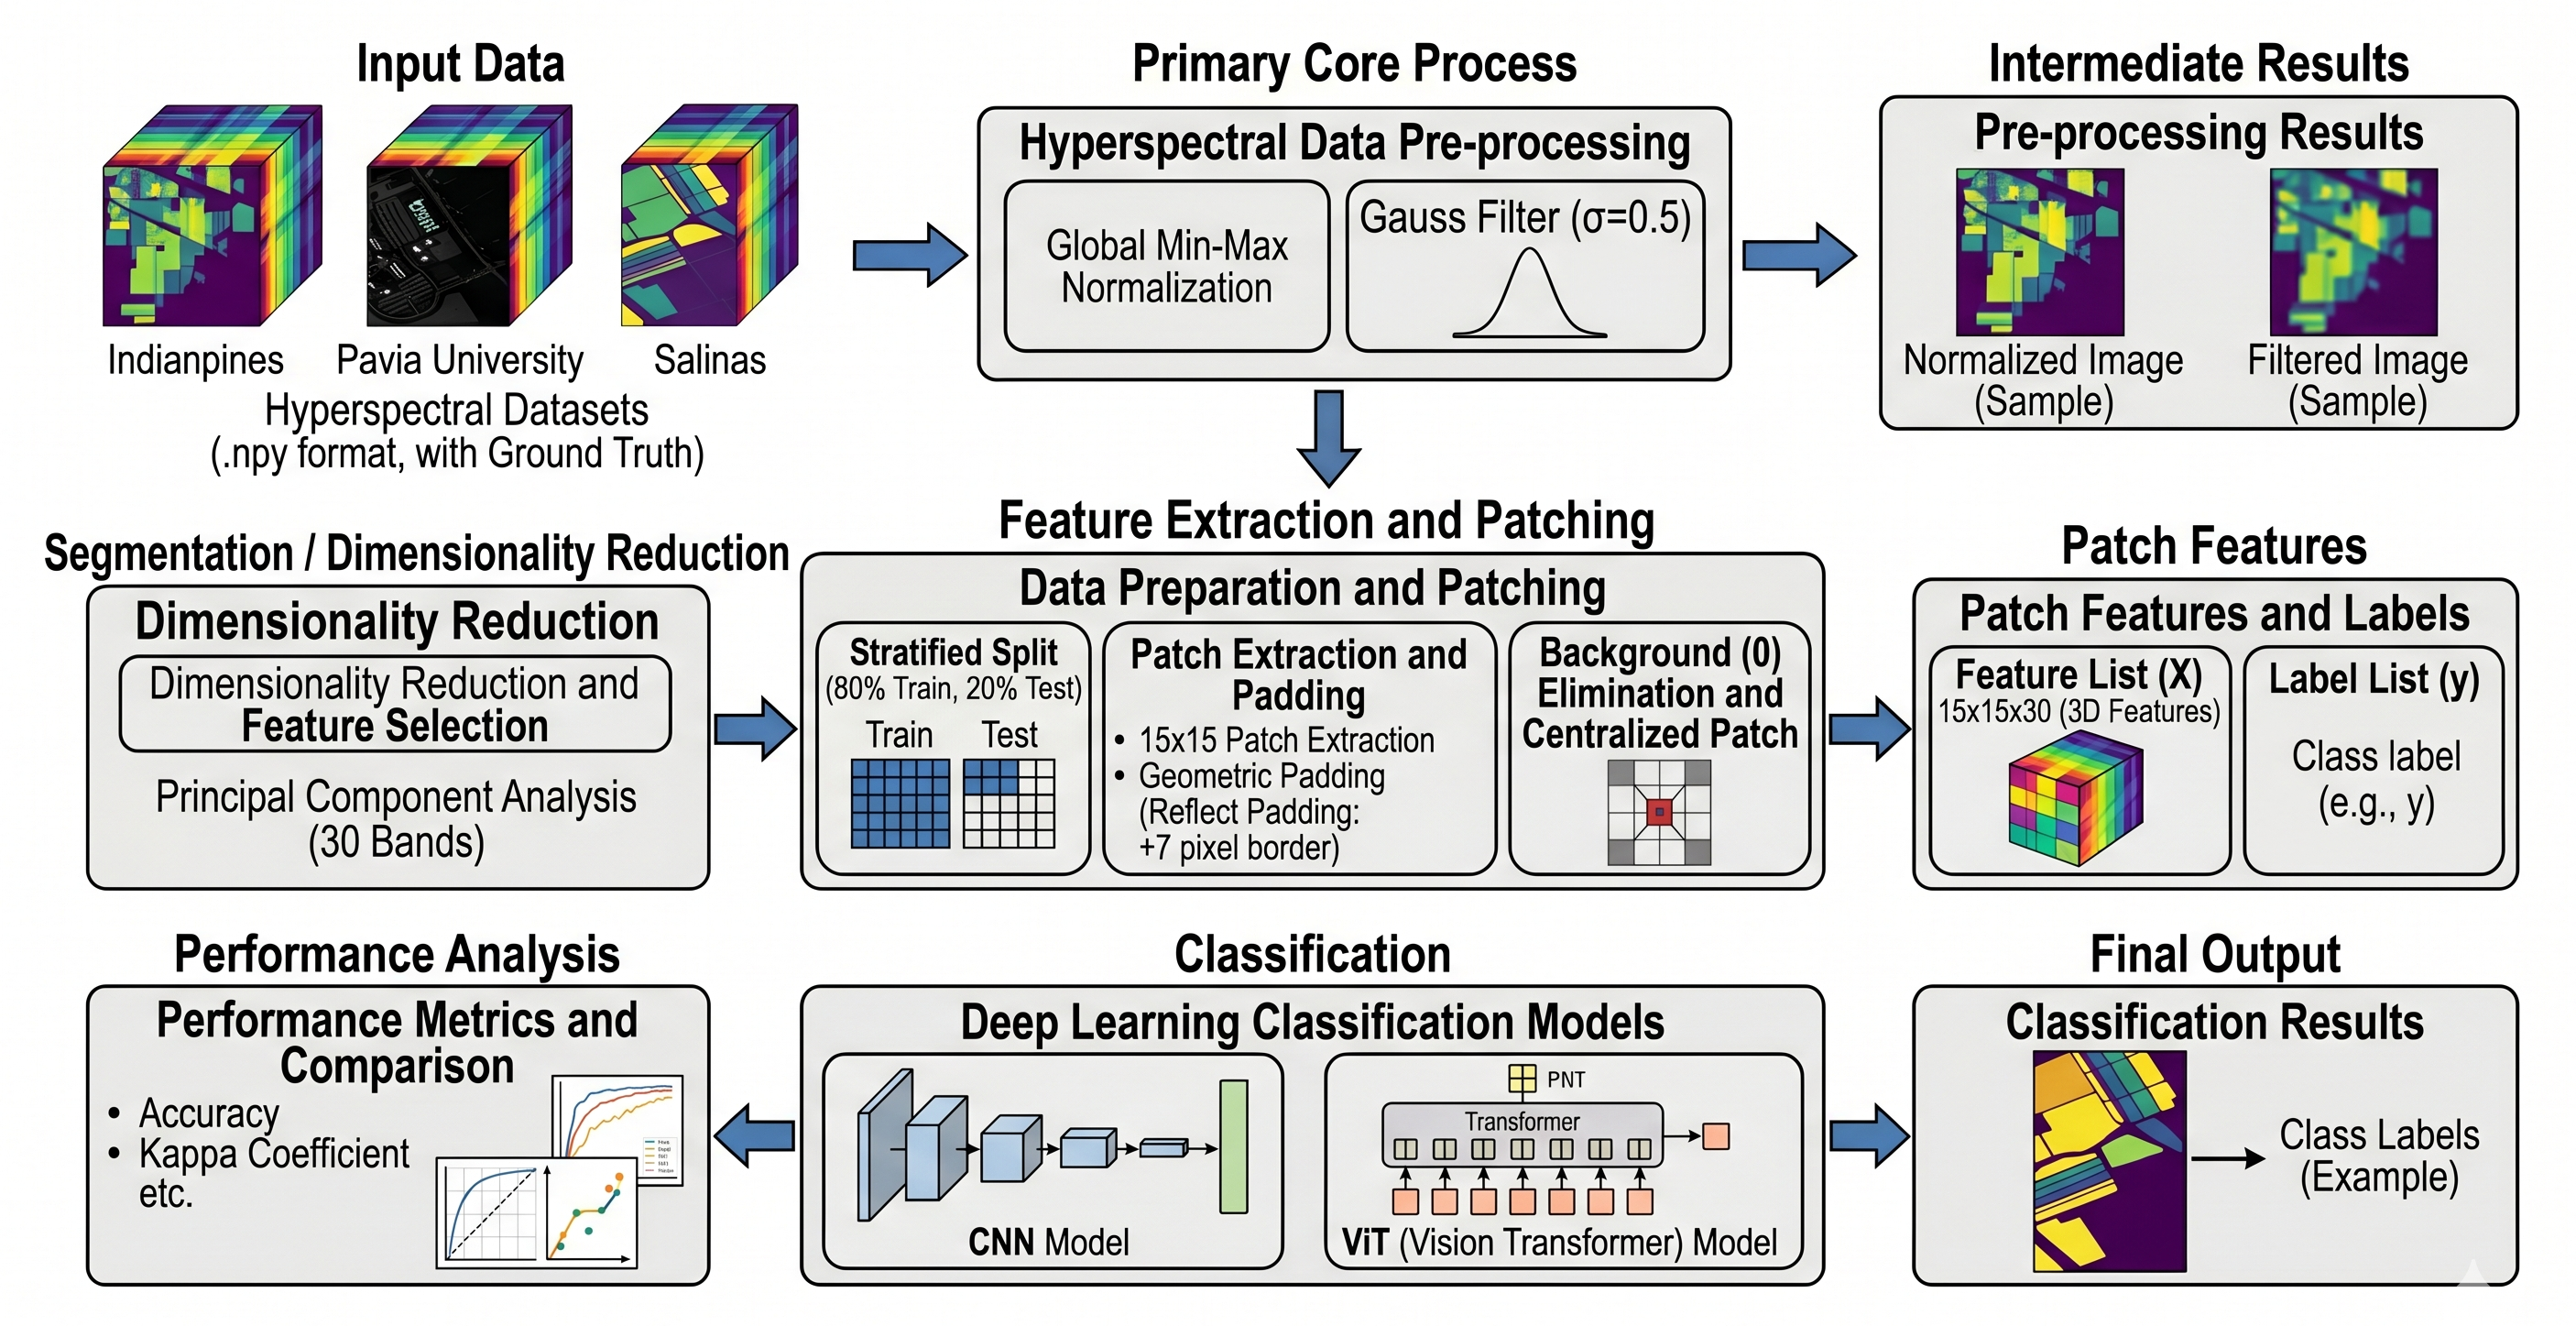
\includegraphics[width=\linewidth]{images/workflow.png}
    \caption{Overall Workflow of the Proposed HSI Classification System}
    \label{fig:workflow}
\end{figure}

\section{Material and Dataset}
Model performance in HSI classification is tightly coupled to dataset characteristics---spatial resolution, class imbalance, and total labeled sample count all shape what a given architecture can learn. Three benchmark datasets from the remote sensing literature are used here, each posing a distinct set of challenges.

\subsection{Dataset Specifications}

\subsubsection{Indian Pines}
Captured by the AVIRIS sensor over north-western Indiana, this dataset spans a $145 \times 145$ pixel grid across 224 spectral reflectance bands and covers 16 vegetation and land-cover classes. Water absorption bands reduce the usable band count to 200 in standard practice \cite{baumgardner2015220}.

\begin{figure}[H]
    \centering
    \begin{minipage}{0.48\textwidth}
        \centering
        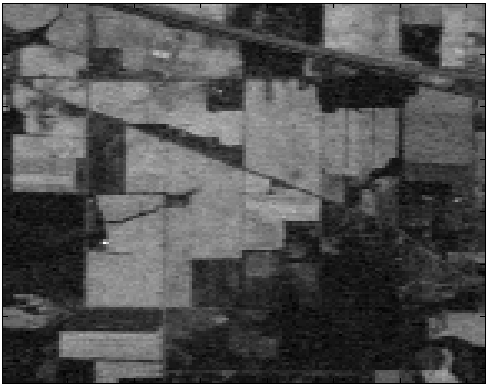
\includegraphics[width=\linewidth]{images/indian_pines_band.png}
        \caption{Indian Pines -- False-color band composite}
        \label{fig:indian_pines_band}
    \end{minipage}
    \hfill
    \begin{minipage}{0.48\textwidth}
        \centering
        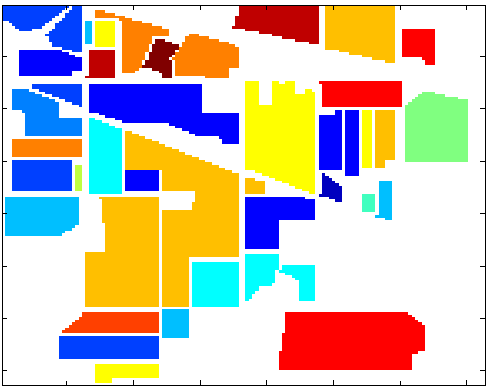
\includegraphics[width=\linewidth]{images/Indian_pines_gt.png}
        \caption{Indian Pines -- Ground truth map}
        \label{fig:indian_pines_gt}
    \end{minipage}
\end{figure}

\begin{table}[H]
    \centering
    \caption{Groundtruth classes for the Indian Pines scene and their respective samples number}
    \label{tab:indian_pines_classes}
    \renewcommand{\arraystretch}{1.2}
    \begin{tabular}{|c|l|c|}
        \hline
        \textbf{\#} & \textbf{Class} & \textbf{Samples} \\ \hline
        1 & Alfalfa & 46 \\ \hline
        2 & Corn-notill & 1428 \\ \hline
        3 & Corn-mintill & 830 \\ \hline
        4 & Corn & 237 \\ \hline
        5 & Grass-pasture & 483 \\ \hline
        6 & Grass-trees & 730 \\ \hline
        7 & Grass-pasture-mowed & 28 \\ \hline
        8 & Hay-windrowed & 478 \\ \hline
        9 & Oats & 20 \\ \hline
        10 & Soybean-notill & 972 \\ \hline
        11 & Soybean-mintill & 2455 \\ \hline
        12 & Soybean-clean & 593 \\ \hline
        13 & Wheat & 205 \\ \hline
        14 & Woods & 1265 \\ \hline
        15 & Buildings-Grass-Trees-Drives & 386 \\ \hline
        16 & Stone-Steel-Towers & 93 \\ \hline
        \multicolumn{2}{|r|}{\textbf{Total}} & \textbf{10249} \\ \hline
    \end{tabular}
\end{table}

\subsubsection{Pavia University}
Acquired by the ROSIS sensor over an urban area in Pavia, Italy, this scene covers $610 \times 340$ pixels across 103 spectral bands. Nine urban land-cover classes---including asphalt, meadows, and self-blocking bricks---make it a demanding multi-class urban benchmark \cite{dell2005pavia}.

\begin{figure}[H]
    \centering
    \begin{minipage}{0.48\textwidth}
        \centering
        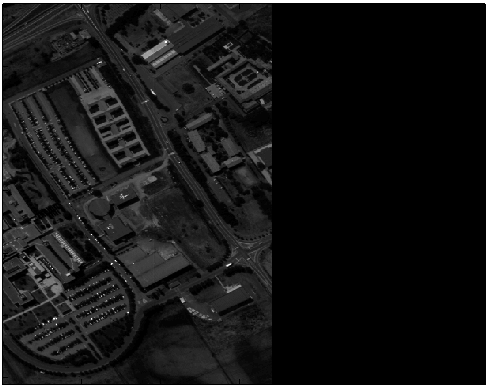
\includegraphics[width=\linewidth]{images/pavia_band.png}
        \caption{Pavia University -- False-color band composite}
        \label{fig:pavia_band}
    \end{minipage}
    \hfill
    \begin{minipage}{0.48\textwidth}
        \centering
        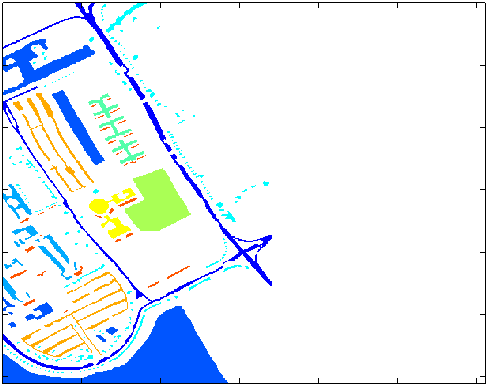
\includegraphics[width=\linewidth]{images/paviau_gt.png}
        \caption{Pavia University -- Ground truth map}
        \label{fig:pavia_gt}
    \end{minipage}
\end{figure}

\begin{table}[H]
    \centering
    \caption{Groundtruth classes for the Pavia University scene and their respective samples number}
    \label{tab:pavia_classes}
    \renewcommand{\arraystretch}{1.2}
    \begin{tabular}{|c|l|c|}
        \hline
        \textbf{\#} & \textbf{Class} & \textbf{Samples} \\ \hline
        1 & Asphalt & 6631 \\ \hline
        2 & Meadows & 18649 \\ \hline
        3 & Gravel & 2099 \\ \hline
        4 & Trees & 3064 \\ \hline
        5 & Painted metal sheets & 1345 \\ \hline
        6 & Bare Soil & 5029 \\ \hline
        7 & Bitumen & 1330 \\ \hline
        8 & Self-Blocking Bricks & 3682 \\ \hline
        9 & Shadows & 947 \\ \hline
        \multicolumn{2}{|r|}{\textbf{Total}} & \textbf{42776} \\ \hline
    \end{tabular}
\end{table}

\subsubsection{Salinas Scene}
Also collected by AVIRIS, this time over Salinas Valley, California, the scene offers the highest spatial resolution of the three datasets: $512 \times 217$ pixels across 224 spectral bands, reduced to 204 after removing water absorption channels \cite{salinas_dataset}.

\begin{figure}[H]
    \centering
    \begin{minipage}{0.48\textwidth}
        \centering
        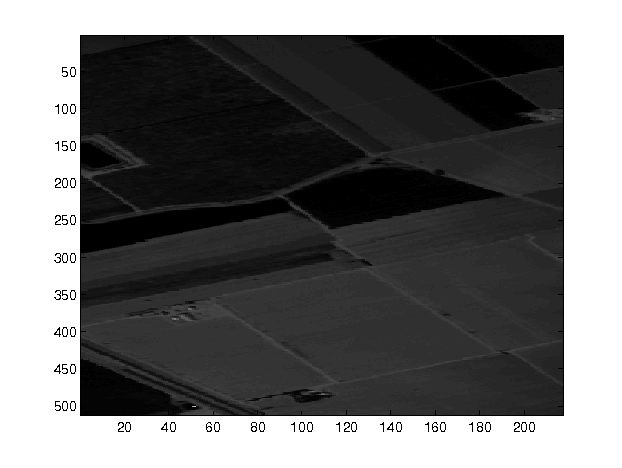
\includegraphics[width=\linewidth]{images/salinas_band.png}
        \caption{Salinas Scene -- False-color band composite}
        \label{fig:salinas_band}
    \end{minipage}
    \hfill
    \begin{minipage}{0.48\textwidth}
        \centering
        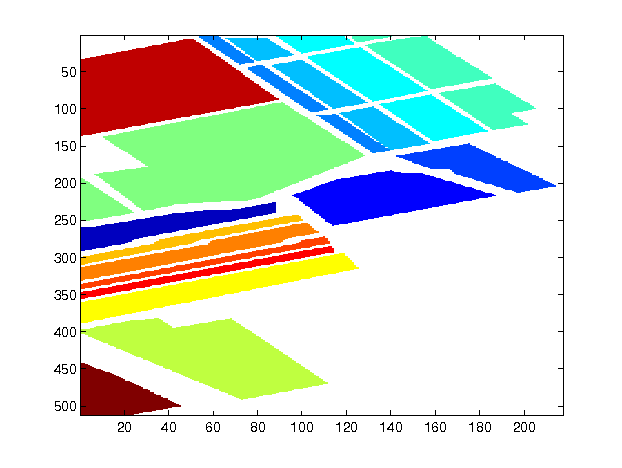
\includegraphics[width=\linewidth]{images/salinas_gt.png}
        \caption{Salinas Scene -- Ground truth map}
        \label{fig:salinas_gt}
    \end{minipage}
\end{figure}

\begin{table}[H]
    \centering
    \caption{Groundtruth classes for the Salinas scene and their respective samples number}
    \label{tab:salinas_classes}
    \renewcommand{\arraystretch}{1.2}
    \begin{tabular}{|c|l|c|}
        \hline
        \textbf{\#} & \textbf{Class} & \textbf{Samples} \\ \hline
        1 & Brocoli\_green\_weeds\_1 & 2009 \\ \hline
        2 & Brocoli\_green\_weeds\_2 & 3726 \\ \hline
        3 & Fallow & 1976 \\ \hline
        4 & Fallow\_rough\_plow & 1394 \\ \hline
        5 & Fallow\_smooth & 2678 \\ \hline
        6 & Stubble & 3959 \\ \hline
        7 & Celery & 3579 \\ \hline
        8 & Grapes\_untrained & 11271 \\ \hline
        9 & Soil\_vinyard\_develop & 6203 \\ \hline
        10 & Corn\_senesced\_green\_weeds & 3278 \\ \hline
        11 & Lettuce\_romaine\_4wk & 1068 \\ \hline
        12 & Lettuce\_romaine\_5wk & 1927 \\ \hline
        13 & Lettuce\_romaine\_6wk & 916 \\ \hline
        14 & Lettuce\_romaine\_7wk & 1070 \\ \hline
        15 & Vinyard\_untrained & 7268 \\ \hline
        16 & Vinyard\_vertical\_trellis & 1807 \\ \hline
        \multicolumn{2}{|r|}{\textbf{Total}} & \textbf{54129} \\ \hline
    \end{tabular}
\end{table}

\subsection{Data Structure and Storage}
All three datasets are represented as 3D hypercubes of shape $H \times W \times B$, where $H$ and $W$ are the spatial dimensions and $B$ is the number of spectral bands. Datasets are stored as NumPy arrays (`.npy`) and loaded in spatial patches during training, which preserves local spatial context while keeping memory consumption tractable.

\begin{figure}[H]
    \centering
    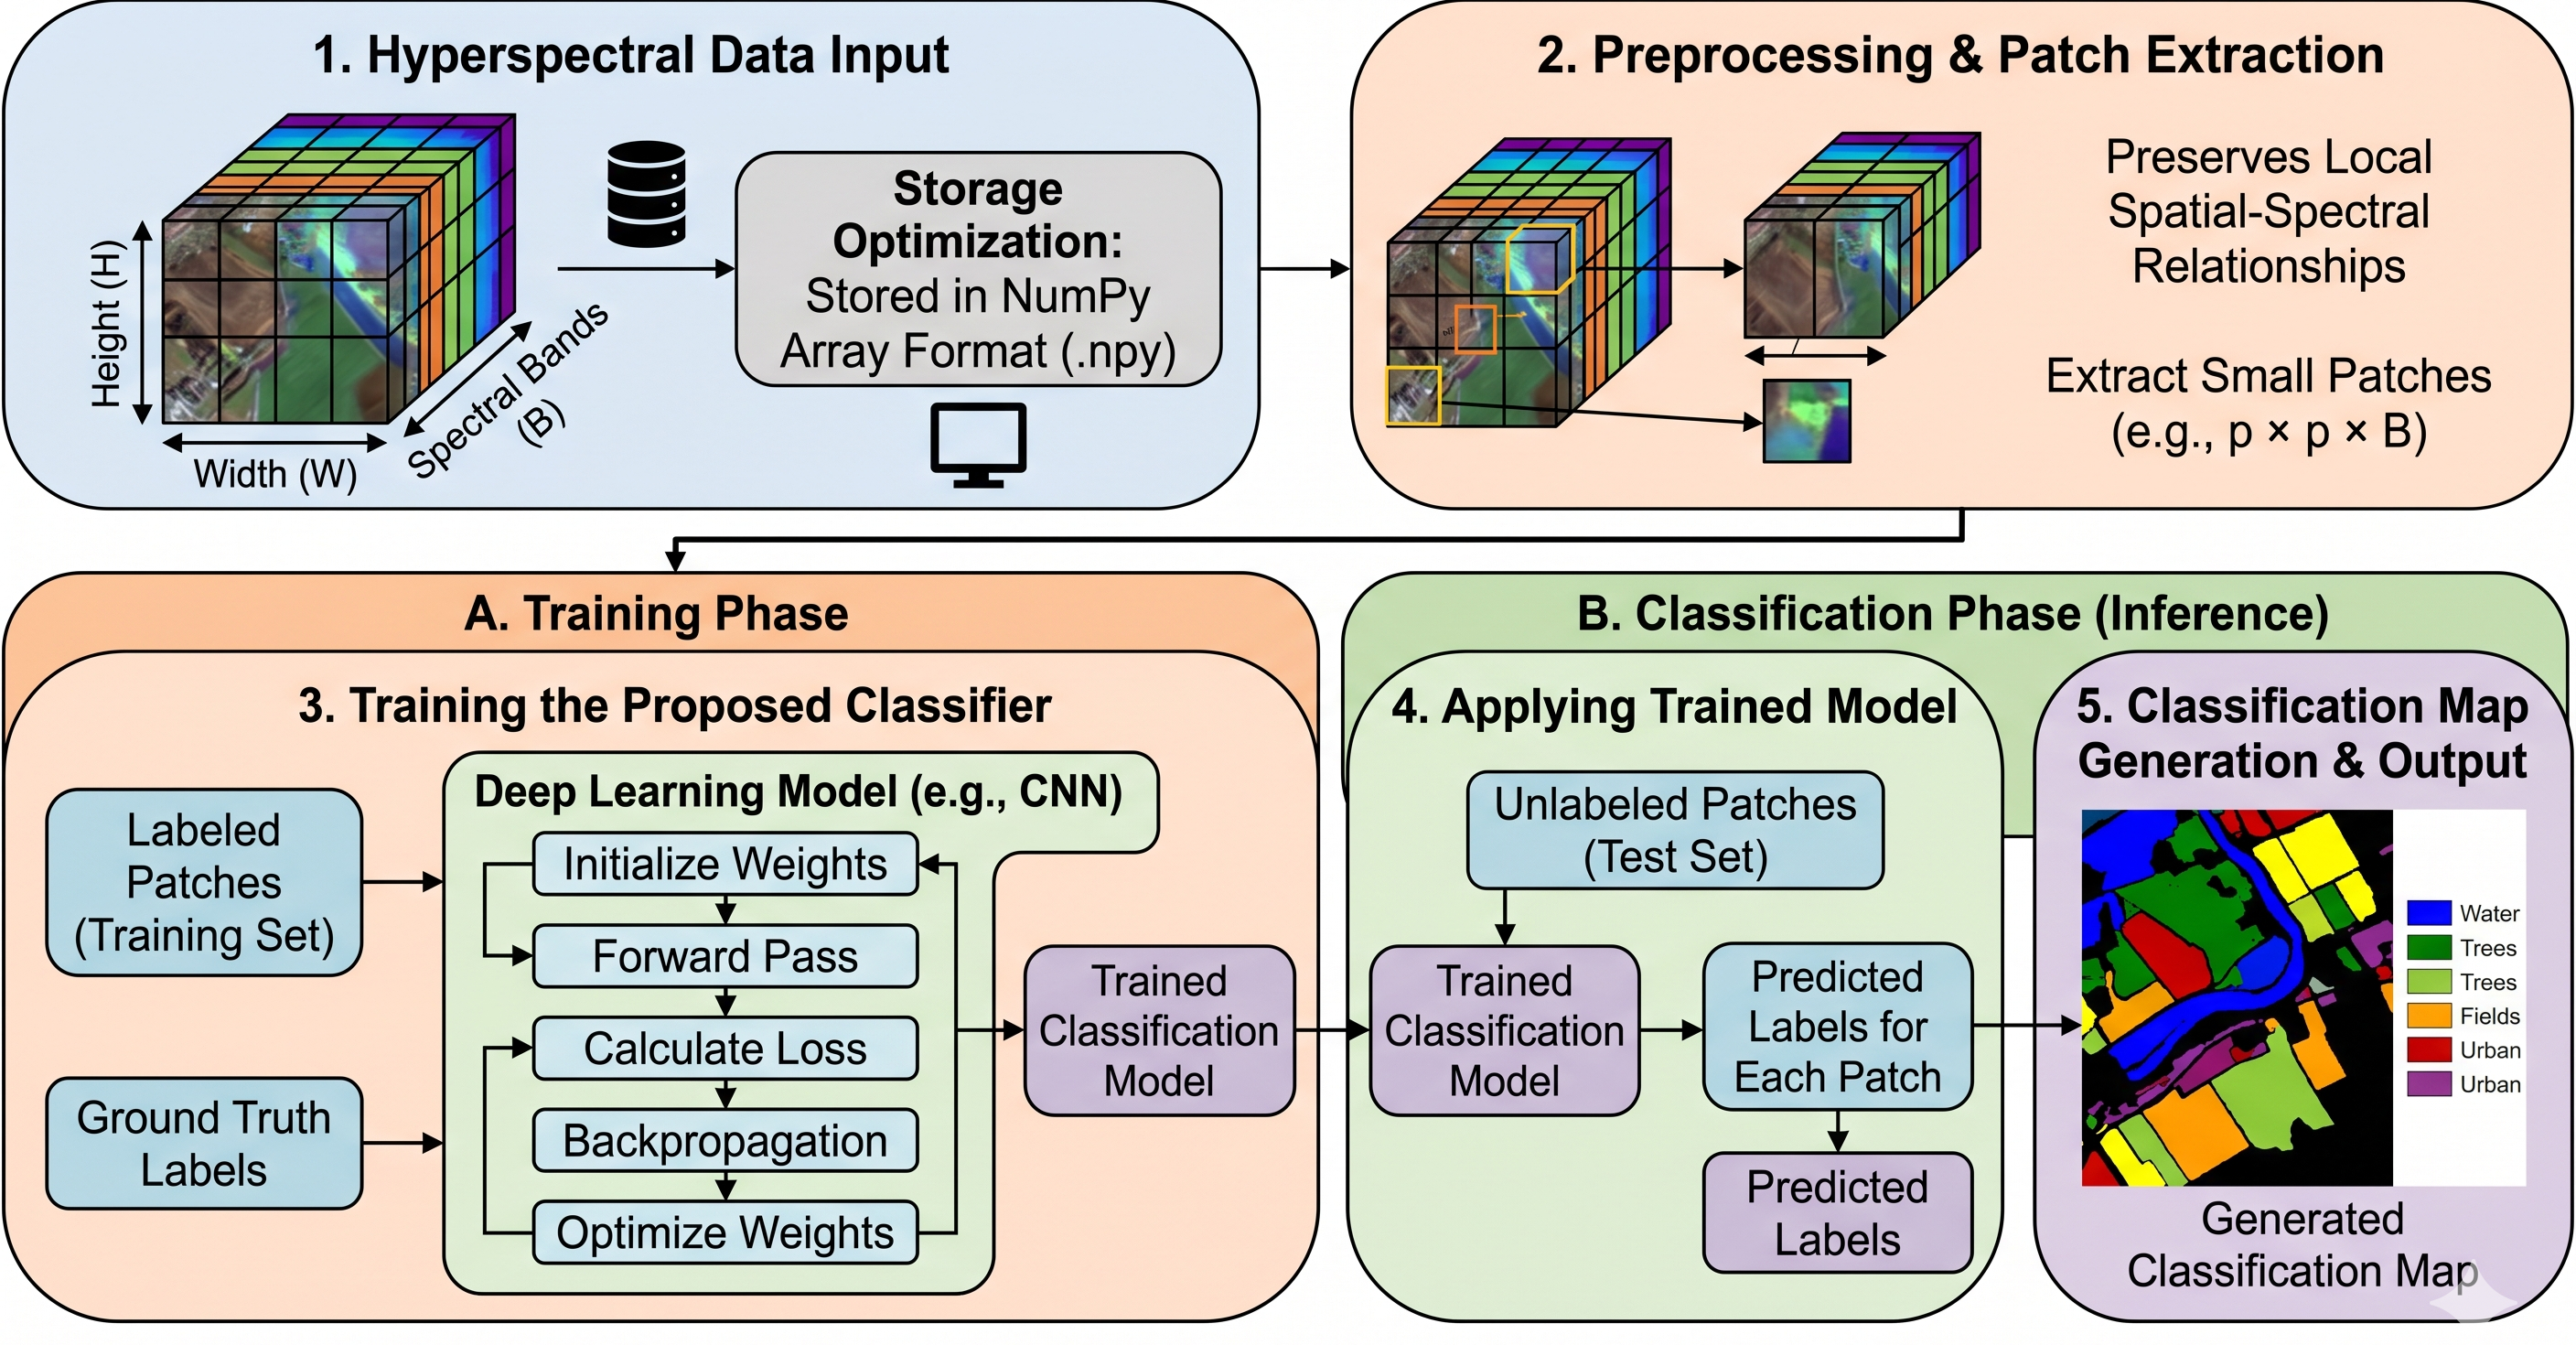
\includegraphics[width=\linewidth]{images/block_diagram.png}
    \caption{General Block Diagram of the Proposed HSI Classification System}
    \label{fig:block_diagram}
\end{figure}

\section{Methodology}
The processing pipeline is structured into three sequential stages: preprocessing, patch-based feature extraction, and the learning phase. Each stage feeds directly into the next, and the design choices at each step are motivated by specific properties of hyperspectral data.

\subsection{Preprocessing and Dimensionality Reduction}
Raw hyperspectral cubes carry hundreds of correlated bands and sensor-induced noise---conditions that inflate training cost and can mislead learned features. Three sequential operations are applied uniformly across all datasets before any model sees the data.

\begin{enumerate}
    \item \textbf{Global Min-Max Normalization:} The raw hypercube is reshaped to a 2D matrix and a single global minimum and maximum is computed across all pixels and all bands. Each value is then rescaled to $[0,1]$ as follows:
    \begin{equation}
        \hat{x} = \frac{x - x_{\min}}{x_{\max} - x_{\min}}
        \label{eq:normalization}
    \end{equation}
    Band-wise normalization was deliberately avoided to preserve the natural variance ratio between bands.

    \item \textbf{Spatial Gaussian Filtering:} A Gaussian filter is applied with $\sigma = 0.5$ along only the spatial axes ($H \times W$) of the normalized hypercube using \texttt{scipy.ndimage.gaussian\_filter} with \texttt{sigma=(0.5, 0.5, 0)} and \texttt{mode='reflect'}. Setting the spectral axis sigma to zero ensures that inter-band relationships remain intact while sensor-induced spatial noise is attenuated.

    \item \textbf{Fixed-Component PCA:} PCA with a fixed $n\_components = 30$ is applied to the filtered data after reshaping it to $(H \times W, B)$. The variance-based threshold (99.5\%) was evaluated first but yielded only 4--5 components for Pavia University and Salinas, which is insufficient for the CNN and ViT input depths. The resulting reduced cube is reshaped back to $(H, W, 30)$ \cite{pedregosa2011scikit}.
\end{enumerate}

\subsection{Patch Extraction and Dataset Splitting}
For each labeled pixel $(r, c)$ where \texttt{gt[r,c] > 0}, a $15 \times 15$ spatial patch is extracted from the PCA-reduced cube, producing a sample of shape $15 \times 15 \times 30$. Background pixels (label $= 0$) are excluded entirely. To allow boundary pixels to serve as valid patch centers, the cube is first padded by $\lfloor 15/2 \rfloor = 7$ pixels on each spatial side using reflect padding.

The resulting patches are split into training and test sets with \texttt{test\_size=0.1}, \texttt{stratify=y}, and \texttt{random\_state=42}, ensuring minority classes are proportionally represented in both splits. The resulting sample counts are given in Table~\ref{tab:split_sizes}.

\begin{table}[H]
    \centering
    \caption{Patch counts after stratified 90/10 train-test split ($15 \times 15 \times 30$)}
    \label{tab:split_sizes}
    \renewcommand{\arraystretch}{1.2}
    \begin{tabular}{|l|c|c|c|}
        \hline
        \textbf{Dataset} & \textbf{Total} & \textbf{Train (90\%)} & \textbf{Test (10\%)} \\ \hline
        Indian Pines     & 10249 & 9224  & 1025  \\ \hline
        Pavia University & 42776 & 38498 & 4278  \\ \hline
        Salinas Scene    & 54129 & 48716 & 5413  \\ \hline
    \end{tabular}
\end{table}

\subsection{Model Architectures}
Two architectures represent complementary inductive biases for spectral-spatial feature learning:
\begin{itemize}
    \item \textbf{3D-CNN:} Three-dimensional convolutional kernels extract spectral and spatial features simultaneously from volumetric patches. Batch normalization and ReLU activations are inserted after each convolutional block to stabilize gradients and prevent vanishing activations \cite{chen2016deep}.
    \item \textbf{Vision Transformer (ViT):} HSI patches are flattened into sequences of linear embeddings, and multi-head self-attention weighs each spectral-spatial token against every other---capturing long-range dependencies that local convolution windows cannot reach \cite{dosovitskiy2020image}.
\end{itemize}

\subsection{Supervised Learning Models}
The supervised paradigm trains exclusively on the labeled portion of the training set. It establishes the performance baseline against which semi-supervised and federated variants are measured.

\subsubsection{2D-CNN Supervised Model}
The 2D-CNN operates on $15 \times 15 \times 30$ patches, treating the 30 PCA components as input channels and applying 2D convolution kernels over the spatial dimensions. This formulation avoids the parameter cost of full volumetric convolution while retaining meaningful spatial-spectral structure.

\subsubsection{3D-CNN Supervised Model}
The 3D-CNN applies volumetric kernels that span both spatial and spectral axes simultaneously, enabling it to model inter-band correlations directly rather than treating spectral bands as independent channels. Batch normalization and dropout mitigate overfitting, which is particularly pronounced when labeled samples are scarce.

\subsubsection{Vision Transformer (ViT) Supervised Model}
The ViT tokenizes each patch into a sequence of linear projections and augments them with positional encodings to retain spatial ordering. Multi-head self-attention then relates every token to every other, giving the model a global receptive field from the first layer. This property has proven competitive on standard HSI benchmarks \cite{dosovitskiy2020image}.

\subsection{Semi-Supervised Learning Models}
Collecting expert-labeled pixel annotations is expensive and slow. Semi-supervised learning sidesteps this bottleneck by treating the large pool of unlabeled pixels as additional training signal. The strategy here pairs self-training with curriculum learning to expand the labeled set iteratively while managing pseudo-label noise.

\subsubsection{Self-Training Strategy}
The self-training mechanism operates through iterative pseudo-labeling:
\begin{enumerate}
    \item Initialize the model using a subset of labeled training samples.
    \item Generate predictions on the unlabeled pool with associated confidence scores.
    \item Incorporate samples exceeding a confidence threshold into the training set with their predicted labels.
    \item Retrain the model on the augmented labeled set.
    \item Repeat until convergence or a maximum iteration limit is reached \cite{triguero2015self}.
\end{enumerate}

\subsubsection{Curriculum Learning Integration}
Curriculum Learning (CL) guides the training process by presenting samples in order of increasing difficulty:
\begin{enumerate}
    \item \textbf{Easy Samples:} Pixels with high spectral purity and clear spatial context are introduced first, allowing the model to learn robust decision boundaries.
    \item \textbf{Medium Samples:} Pixels with moderate spectral-spatial characteristics are gradually introduced as the model gains confidence.
    \item \textbf{Difficult Samples:} Boundary pixels and spectrally ambiguous samples are presented in later epochs to refine the decision boundaries \cite{bengio2009curriculum}.
\end{enumerate}

\subsubsection{2D-CNN Semi-Supervised Model}
The architecture is identical to its supervised counterpart. What changes is the training set: self-training iteratively adds high-confidence pseudo-labeled patches, and curriculum learning controls the order in which those additions are presented, dampening the effect of early-stage label noise.

\subsubsection{3D-CNN Semi-Supervised Model}
Unlabeled samples admitted through self-training expose the 3D-CNN to a wider range of spectral-spatial patterns than the labeled set alone provides. Curriculum scheduling prevents the volumetric kernels from overfitting to the noisiest pseudo-labels encountered in early iterations.

\subsubsection{Vision Transformer (ViT) Semi-Supervised Model}
The global receptive field of the self-attention mechanism makes the ViT naturally suited to semi-supervised settings: it can relate high-confidence pseudo-labeled tokens to labeled ones across the full spatial extent of a patch, rather than relying solely on local neighborhood agreement.

\subsection{Federated Learning Models}
Federated learning trains a shared global model without ever moving raw data to a central server---each client trains locally and contributes only weight updates. In this project, federated learning is simulated through a server-client architecture in which three geographically distinct datasets stand in for independent client institutions \cite{mcmahan2017communication}.

\subsubsection{Federated Learning Framework}
The federated learning process follows the Federated Averaging (FedAvg) algorithm:
\begin{enumerate}
    \item Initialize a global model at the central server.
    \item Each client downloads the global model weights and trains locally on its own hyperspectral dataset for a fixed number of epochs.
    \item Clients upload their updated model weights to the server (not raw data, preserving privacy).
    \item The server aggregates weights from all participating clients through averaging.
    \item The updated global model is redistributed to clients for the next round.
    \item Repeat for multiple communication rounds until convergence.
\end{enumerate}

\subsubsection{2D-CNN Federated Model}
Each client (Indian Pines, Pavia University, and Salinas in this simulation) trains an identical 2D-CNN locally under shared hyperparameters. Weight averaging at the server fuses the dataset-specific spatial patterns learned at each site into a single global model without exposing any client's raw pixels.

\subsubsection{3D-CNN Federated Model}
The 3D-CNN's volumetric kernels encode dataset-specific spectral correlations during local training. After aggregation, the global model inherits a richer spectral vocabulary than any single-dataset model could develop---particularly valuable in remote sensing, where data is routinely distributed across multiple acquisition campaigns and sensor configurations.

\subsubsection{Vision Transformer (ViT) Federated Model}
Transformer attention weights encode the local data distribution of each client site. Their aggregation at the server produces a global self-attention mechanism capable of handling the heterogeneous spectral-spatial statistics that arise when different sensors observe different geographic regions.

\subsubsection{Privacy and Communication Efficiency}
Keeping raw hyperspectral data at client locations is the primary privacy guarantee of federated learning, but communication overhead between clients and the server is a practical constraint. Three measures address this:
\begin{itemize}
    \item \textbf{Gradient Compression:} Model weights are compressed before transmission to reduce bandwidth requirements.
    \item \textbf{Local Training Epochs:} Each client performs multiple local training epochs (typically 5--10) before communicating with the server, reducing the total number of communication rounds.
    \item \textbf{Asynchronous Aggregation:} The server aggregates updates from whichever clients respond first rather than waiting for all participants, reducing wall-clock training time.
\end{itemize}

\subsection{Comparative Learning Paradigm Summary}
The three paradigms each address labeled data scarcity from a different angle. Table~\ref{tab:learning_paradigms} summarizes their key characteristics.

\begin{table}[H]
    \centering
    \caption{Comparison of Supervised, Semi-Supervised, and Federated Learning Paradigms}
    \label{tab:learning_paradigms}
    \renewcommand{\arraystretch}{1.3}
    \begin{tabular}{|l|c|c|c|}
        \hline
        \textbf{Characteristic} & \textbf{Supervised} & \textbf{Semi-Supervised} & \textbf{Federated} \\ \hline
        \textbf{Data Requirement} & Fully Labeled & Partial Labels & Local Data Privacy \\ \hline
        \textbf{Scalability} & Centralized & Centralized & Distributed \\ \hline
        \textbf{Communication Cost} & None & None & High \\ \hline
        \textbf{Privacy Protection} & Limited & Limited & High \\ \hline
        \textbf{Typical Accuracy} & Baseline & Enhanced & Comparable \\ \hline
    \end{tabular}
\end{table}

\begin{figure}[H]
    \centering
    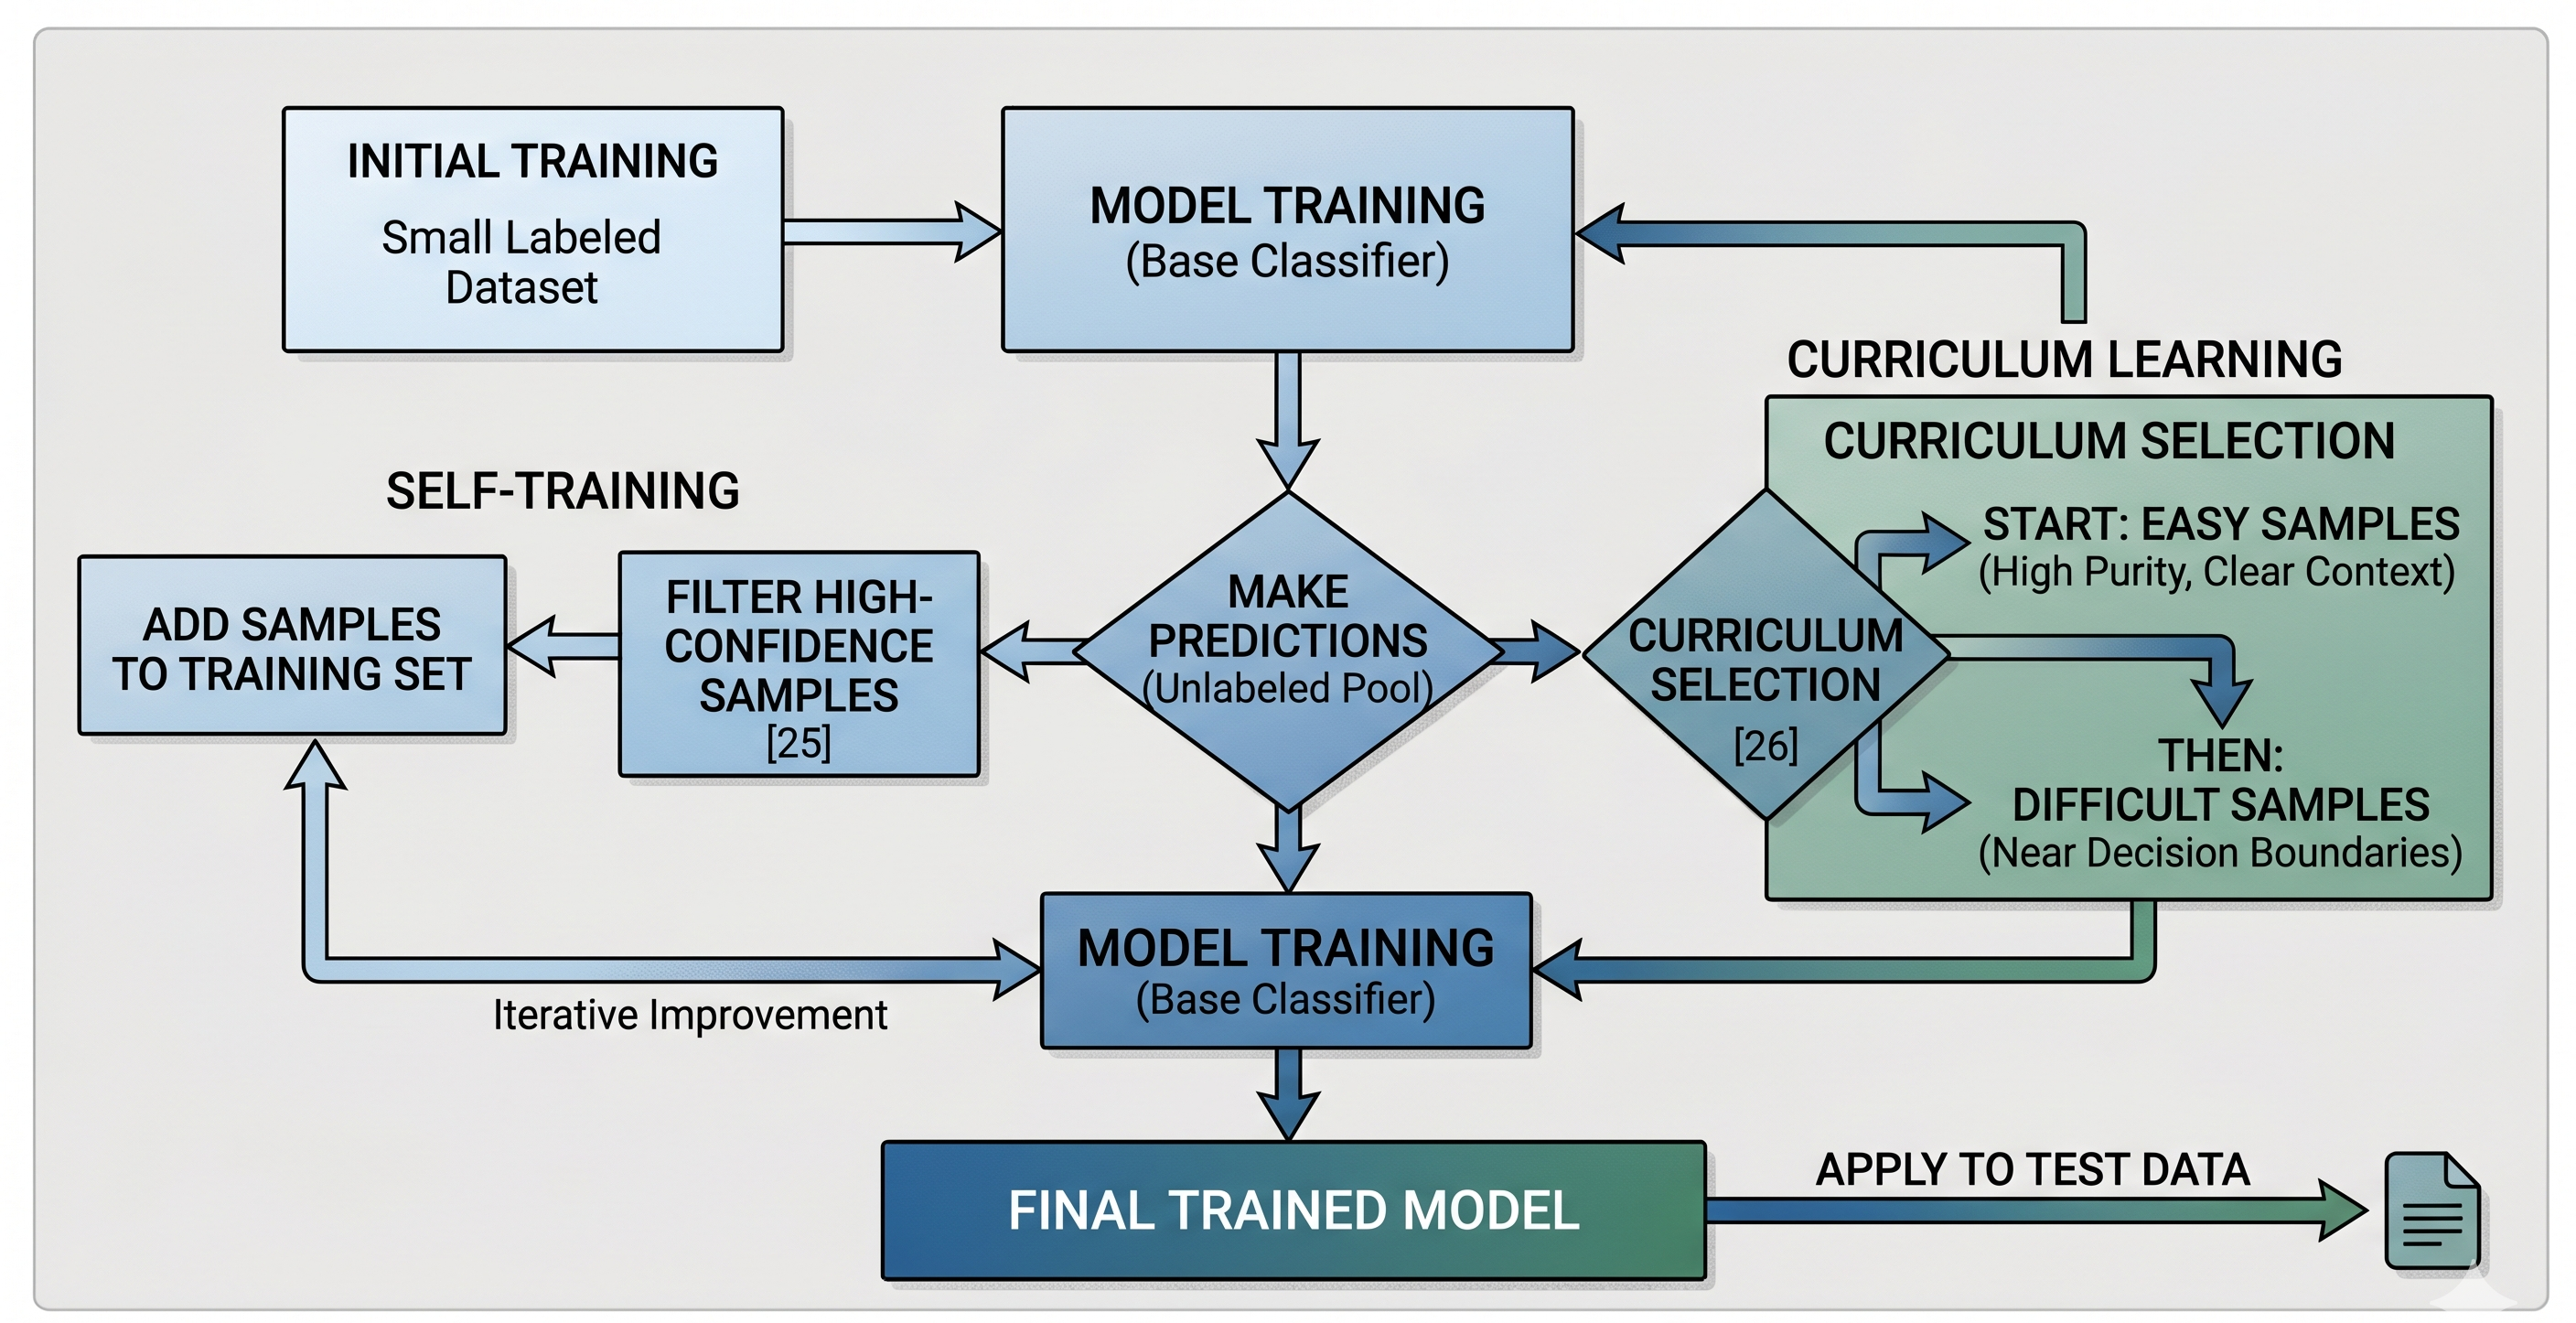
\includegraphics[width=\linewidth]{images/SSL_flowchart.png}
    \caption{Flowchart of the Semi-Supervised Learning Strategy}
    \label{fig:flowchart}
\end{figure}

\subsection{Evaluation Metrics}
Five standard metrics quantify classification performance. Let $TP_c$, $FP_c$, and $FN_c$ denote the true positives, false positives, and false negatives for class $c$, and let $N$ be the total number of test samples.

\begin{itemize}
    \item \textbf{Overall Accuracy (OA):} The ratio of correctly classified pixels to the total number of test pixels:
    \begin{equation}
        \text{OA} = \frac{\sum_{c} TP_c}{N}
    \end{equation}

    \item \textbf{Precision:} The fraction of pixels predicted as class $c$ that truly belong to class $c$, averaged across all classes (macro):
    \begin{equation}
        \text{Precision} = \frac{1}{C} \sum_{c=1}^{C} \frac{TP_c}{TP_c + FP_c}
    \end{equation}

    \item \textbf{Recall:} The fraction of true class-$c$ pixels that are correctly identified:
    \begin{equation}
        \text{Recall} = \frac{1}{C} \sum_{c=1}^{C} \frac{TP_c}{TP_c + FN_c}
    \end{equation}

    \item \textbf{F1-Score:} The harmonic mean of Precision and Recall:
    \begin{equation}
        \text{F1} = \frac{2 \cdot \text{Precision} \cdot \text{Recall}}{\text{Precision} + \text{Recall}}
    \end{equation}

    \item \textbf{Cohen's Kappa ($\kappa$):} A metric that corrects Overall Accuracy for agreement expected by chance. Given the observed accuracy $p_o$ and the chance agreement $p_e$:
    \begin{equation}
        \kappa = \frac{p_o - p_e}{1 - p_e}
    \end{equation}
    A value of $\kappa = 1$ indicates perfect classification; $\kappa = 0$ is equivalent to random guessing.
\end{itemize}

\subsection{GUI and Multithreading Integration}
The trained models are exposed through a standalone PyQt6 desktop application. Model inference runs in a dedicated worker thread, decoupled from the main UI event loop, so the interface remains fully responsive while the deep learning pipeline processes large hyperspectral hypercubes in the background.
